\documentclass{article}

\usepackage[margin=0.75in]{geometry}

\usepackage{polski}
\usepackage[utf8]{inputenc}
\usepackage{graphicx} % Required for inserting images
\usepackage{amsmath}
\usepackage{amssymb}
\usepackage{float}
\usepackage[shortlabels]{enumitem}
\usepackage{matlab-prettifier}
\usepackage{tcolorbox}

\DeclareMathOperator*{\argmax}{arg\,max}

\title{
    Teoria Sterowania\\
    \Large Metoda Lapunowa
}
\author{Maciej Różewicz}
\date{\today}

\makeatletter         
\def\@maketitle{
\raggedright
\begin{center}
    
\includegraphics[width=0.55\linewidth]{fig/agh_logo.PNG}\\[8ex]
\end{center}
\begin{center}
    {\huge \bfseries \sffamily \@title }\\[4ex] 
    {\large  \@author}\\[4ex] 
    \@date\\[8ex]
\end{center}}
\makeatother

\begin{document}
\maketitle

%%%%%%%%%%%%%%%%%%%%%%%%%%%%%%%%%%%%%%%%%%%%%%%%%%%%%%%%%%%%
\newpage
\section{Wprowadzenie}
W ćwiczeniu tym rozważamy nieliniowe układy dynamiczne, które mogą być opisane skończonym układem równań różniczkowych zwyczajnych w postaci:
\begin{equation}\label{eq:sys}
    \dot{x}(t) = f(t, x)
\end{equation}
gdzie: $t\in \mathbb{R}$, $x\in\mathbb{R}^{n}$ i $f: \mathbb{R} \times \mathbb{R}^{n} \rightarrow \mathbb{R}^{n}$.

\subsection{Punkty równowagi i stabilność w sensie Lapunowa}

W tej sekcji znajduje się definicje potrzebnych nam pojęć z zakresu stabilności.

\textbf{Definicja 1}
\textbf{Punktem równowagi} układu (\ref{eq:sys}) nazywamy każdy stan $x_{e}$, dla którego $\dot{x}(t) = f(t, x_{e}) = 0$ dla każdego $t>t_{0}$.

\textbf{Definicja 2}
Punkt równowagi $x_{e}$ jest nazywany \textbf{izolowanym punktem równowagi}, jeśli istnieje jego otoczenie, niezawierające żadnych innych punktów równowagi.

\textbf{Definicja 3}
Jeżeli istnieje zmienne w czasie rozwiązanie równania (\ref{eq:sys}) spełniające warunek
$$
    x(t+T) = x(t)
$$
dla pewnego $T>0$ i każdego $t>t_{0}$, to nazywamy je \textbf{cyklem granicznym}. Trajektoria w przestrzeni stanów, odpowiadająca cyklowi granicznemu, ma postać zamkniętej krzywej.

\begin{tcolorbox}[colback=green!5, colframe=green!75!black, title=Przykład]
Przykładem cyklu granicznego jest tak zwany oscylator Van der Pola:
\begin{equation}\label{eq:van_der_pol}
    \left\{
    \begin{array}{l}
         \dot{x}_{1} = x_{2}\\
         \dot{x}_{2} = -x_{1} + (1-x_{1})x_{2} 
    \end{array}
    \right\}.
\end{equation}
Na rysunku (\ref{fig:van_der_pol}) przedstawiono portret tego układu, gdzie wyraźnie widoczny jest występujący tam cykl graniczny.
\begin{figure}[H]
    \centering
    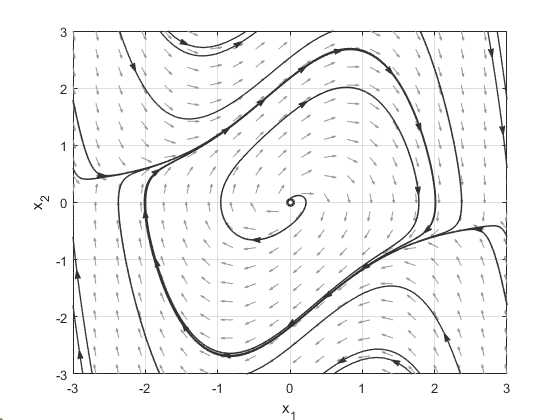
\includegraphics[width=0.5\linewidth]{fig/van_der_pol.png}
    \caption{Portret fazowy dla oscylatora Van der Pola (równanie \ref{eq:van_der_pol}).}
    \label{fig:van_der_pol}
\end{figure}
\end{tcolorbox}

Liczba cykli granicznych nie musi być ograniczona tylko do jednego' lub nawet
skończonej liczby - może być ich dowolna ilość, nawet nieskończenie wiele.

\begin{tcolorbox}[colback=green!5, colframe=green!75!black, title=Przykład]
Rozważmy układ (\ref{eq:cykle_graniczne}):
\begin{equation}\label{eq:cykle_graniczne}
    \left\{
    \begin{array}{l}
         \dot{x}_{1} = x_{2}\\
         \dot{x}_{2} = -\left[ 1 + \sin{(x_{1}^{2}+x_{2}^{2})} \right] x_{2} - x_{1}
    \end{array}
    \right\}.
\end{equation}
Stosunkowo łatwo zauważyć, że cykl graniczny będzie istniał dla każdego $x_{1}$ i $x_{2}$ spełniającego równanie:
$$
    1 + \sin{(x_{1}^{2} + x_{2}^{2})} = 0.
$$
Zatem musi zachodzić:
$$
    x_{1}^{2} + x_{2}^{2} = \frac{3}{2}\pi + 2n\pi.
$$
Portret fazowy tego układu pokazany jest na rysunku (\ref{fig:cykle_graniczne}).
\begin{figure}[H]
    \centering
    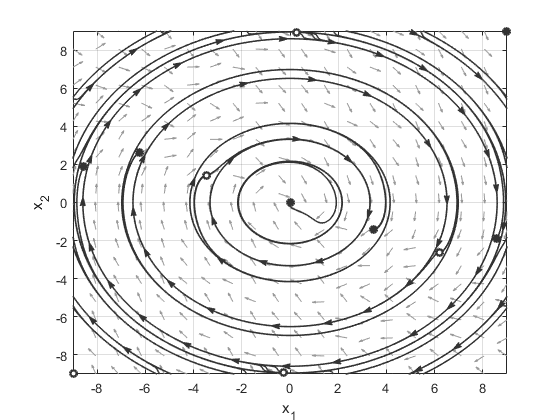
\includegraphics[width=0.5\linewidth]{fig/cykle_graniczne.png}
    \caption{Portret fazowy dla układu opisanego układem równań \ref{eq:cykle_graniczne}.}
    \label{fig:cykle_graniczne}
\end{figure}
\end{tcolorbox}

\textbf{Definicja 4}
Punkt równowagi $x_{e}$  układu (\ref{eq:sys}) nazywamy \textbf{stabilnym} w sensie Lapunowa, jeśli dla dowolnych $t_{0} > 0$, $\epsilon > 0$ istnieje liczba $\delta_{\epsilon} > 0$ (może zależeć od $t_{0}$ i $\epsilon$) taka, że:
\begin{equation}\label{eq:lyap_def}
    \lVert x_{e} - x_{0} \rVert < \delta_{\epsilon}(t_{0}) \implies \lVert x_{e} - x(t;t_{0},x_{0}) \rVert < \epsilon.
\end{equation}
%Układ ten ma jeden punkt równowagi w początku układu współrzędnych, a jego obszarem atrakcji jest cała płaszczyzna $\mathbb{R}^{2}$, lecz nie jest on stabilny. Ponieważ nie można dobrać takiego $\delta$, aby implikacja (\ref{eq:lyap_def}) była spełniona.

Interpretacja stabilność w sensie Lapunowa "krok po kroku":
\begin{description}
    \item[Krok 1] Punkt równowagi $x_e$ nazywamy \textbf{stabilnym} w sensie Lapunowa, jeżeli dla każdej kuli o wymyślonym przez nas promieniu $\epsilon$ ...
    \begin{figure}[H]
    \centering
    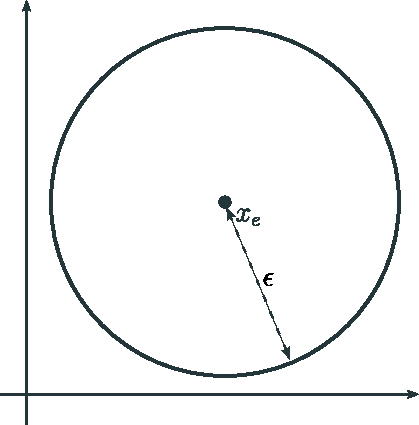
\includegraphics[width=0.3\linewidth]{fig/StabilnoscLapunowaTS2Krok1.pdf}
    \end{figure}
    \item[Krok 2] ... można znaleźć kulę o promieniu $\delta_{\epsilon}$, ...
    \begin{figure}[H]
    \centering
    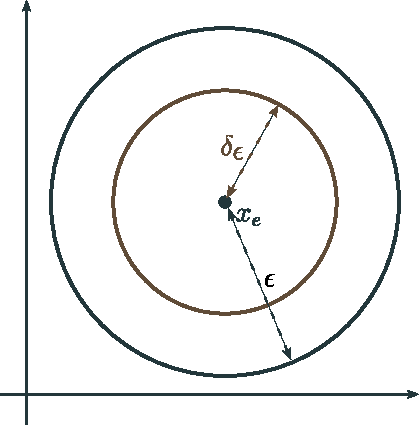
\includegraphics[width=0.3\linewidth]{fig/StabilnoscLapunowaTS2Krok2.pdf}
    \end{figure}
    \item[Krok 3] ... aby każda trajektoria fazowa układu rozpoczynająca się w jakimkolwiek punkcie $x_0$ leżącym w kuli o promieniu $\delta_{\epsilon}$ ...
    \begin{figure}[H]
    \centering
    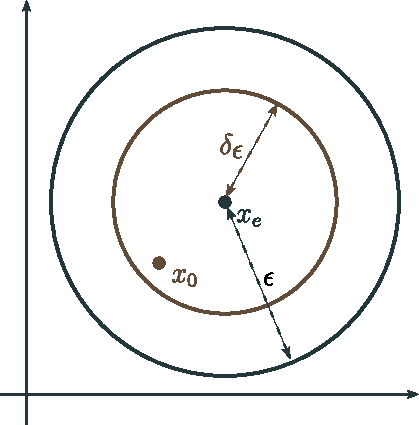
\includegraphics[width=0.3\linewidth]{fig/StabilnoscLapunowaTS2Krok3.pdf}
    \end{figure} 
    \item[Krok 4] ... zawsze pozostała wewnątrz kuli o promieniu $\epsilon$.
    \begin{figure}[H]
    \centering
    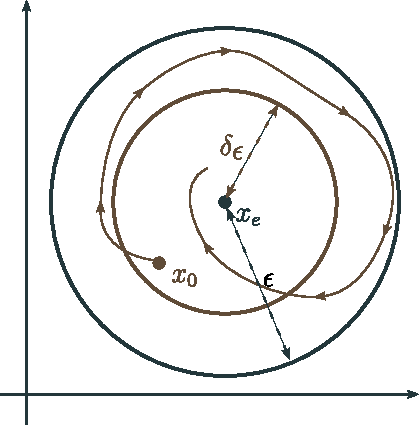
\includegraphics[width=0.3\linewidth]{fig/StabilnoscLapunowaTS2Krok4Stabilny.pdf}
    \caption{Stabilny punkt równowagi - interpretacja geometryczna.}
    \label{fig:punkt_stabilny_lapunowa_interpretacja}
    \end{figure} 
\end{description}

\textbf{Definicja 5}
Punkt równowagi $x_{e}$ układu (\ref{eq:sys}) nazywamy \textbf{niestabilnym}, jeśli nie jest stabilny w sensie definicji 4.
\begin{figure}[H]
\centering
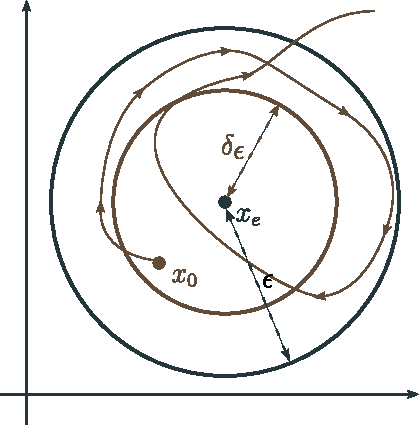
\includegraphics[width=0.3\linewidth]{fig/StabilnoscLapunowaTS2Krok4Niestabilny.pdf}
\caption{Niestabilny punkt równowagi - istnieją takie $\epsilon$, że nie da się znaleźć $\delta_{\epsilon}$, dla którego stan pozostanie w kuli o promieniu $\epsilon$.} 
\label{fig:punkt_niestabilny_lapunowa_interpretacja}
\end{figure} 

\textbf{Definicja 6}
Punkt równowagi $x_{e}$ układu (\ref{eq:sys}) nazywamy \textbf{jednostajnie stabilnym}, jeśli $\delta_{\epsilon}$ z definicji 4 jest niezależne od czasu początkowego $t_{0}$.

\textbf{Definicja 7}
Punkt równowagi $x_{e}$  układu (\ref{eq:sys}) nazywamy \textbf{stabilnym asymptotycznie}, jeśli jest stabilny (w sensie definicji 4) oraz istnieje $\delta_{\epsilon} > 0$ takie że:
\begin{equation}\label{eq:as}
    \lVert x_{e} - x_{0} \rVert < \delta_{\epsilon}(t_{0}) \implies 
 \lim_{t\rightarrow\infty}\lVert x_{e} - x(t;t_{0},x_{0}) \rVert = 0.
\end{equation}

\begin{figure}[H]
\centering
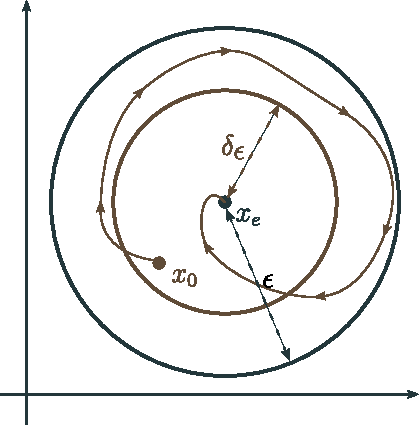
\includegraphics[width=0.3\linewidth]{fig/StabilnoscLapunowaTS2Krok4StabilnyAsymptotycznie.pdf}
\caption{Punkt stabilny asymptotycznie - nie tylko da się znaleźć $\delta_{\epsilon}$ dla każdego $\epsilon$, ale dodatkowo jeszcze stan $x$ zbiega do punktu $x_e$.}
\label{fig:punkt_stabilny_asymptotycznie_lapunowa_interpretacja}
\end{figure} 

\begin{tcolorbox}[colback=green!5, colframe=green!75!black, title=Przykład 1]
Rozważmy oscylator o portrecie fazowym jak na rysunku \ref{fig:example_oscillator}.
\begin{figure}[H]
    \centering
    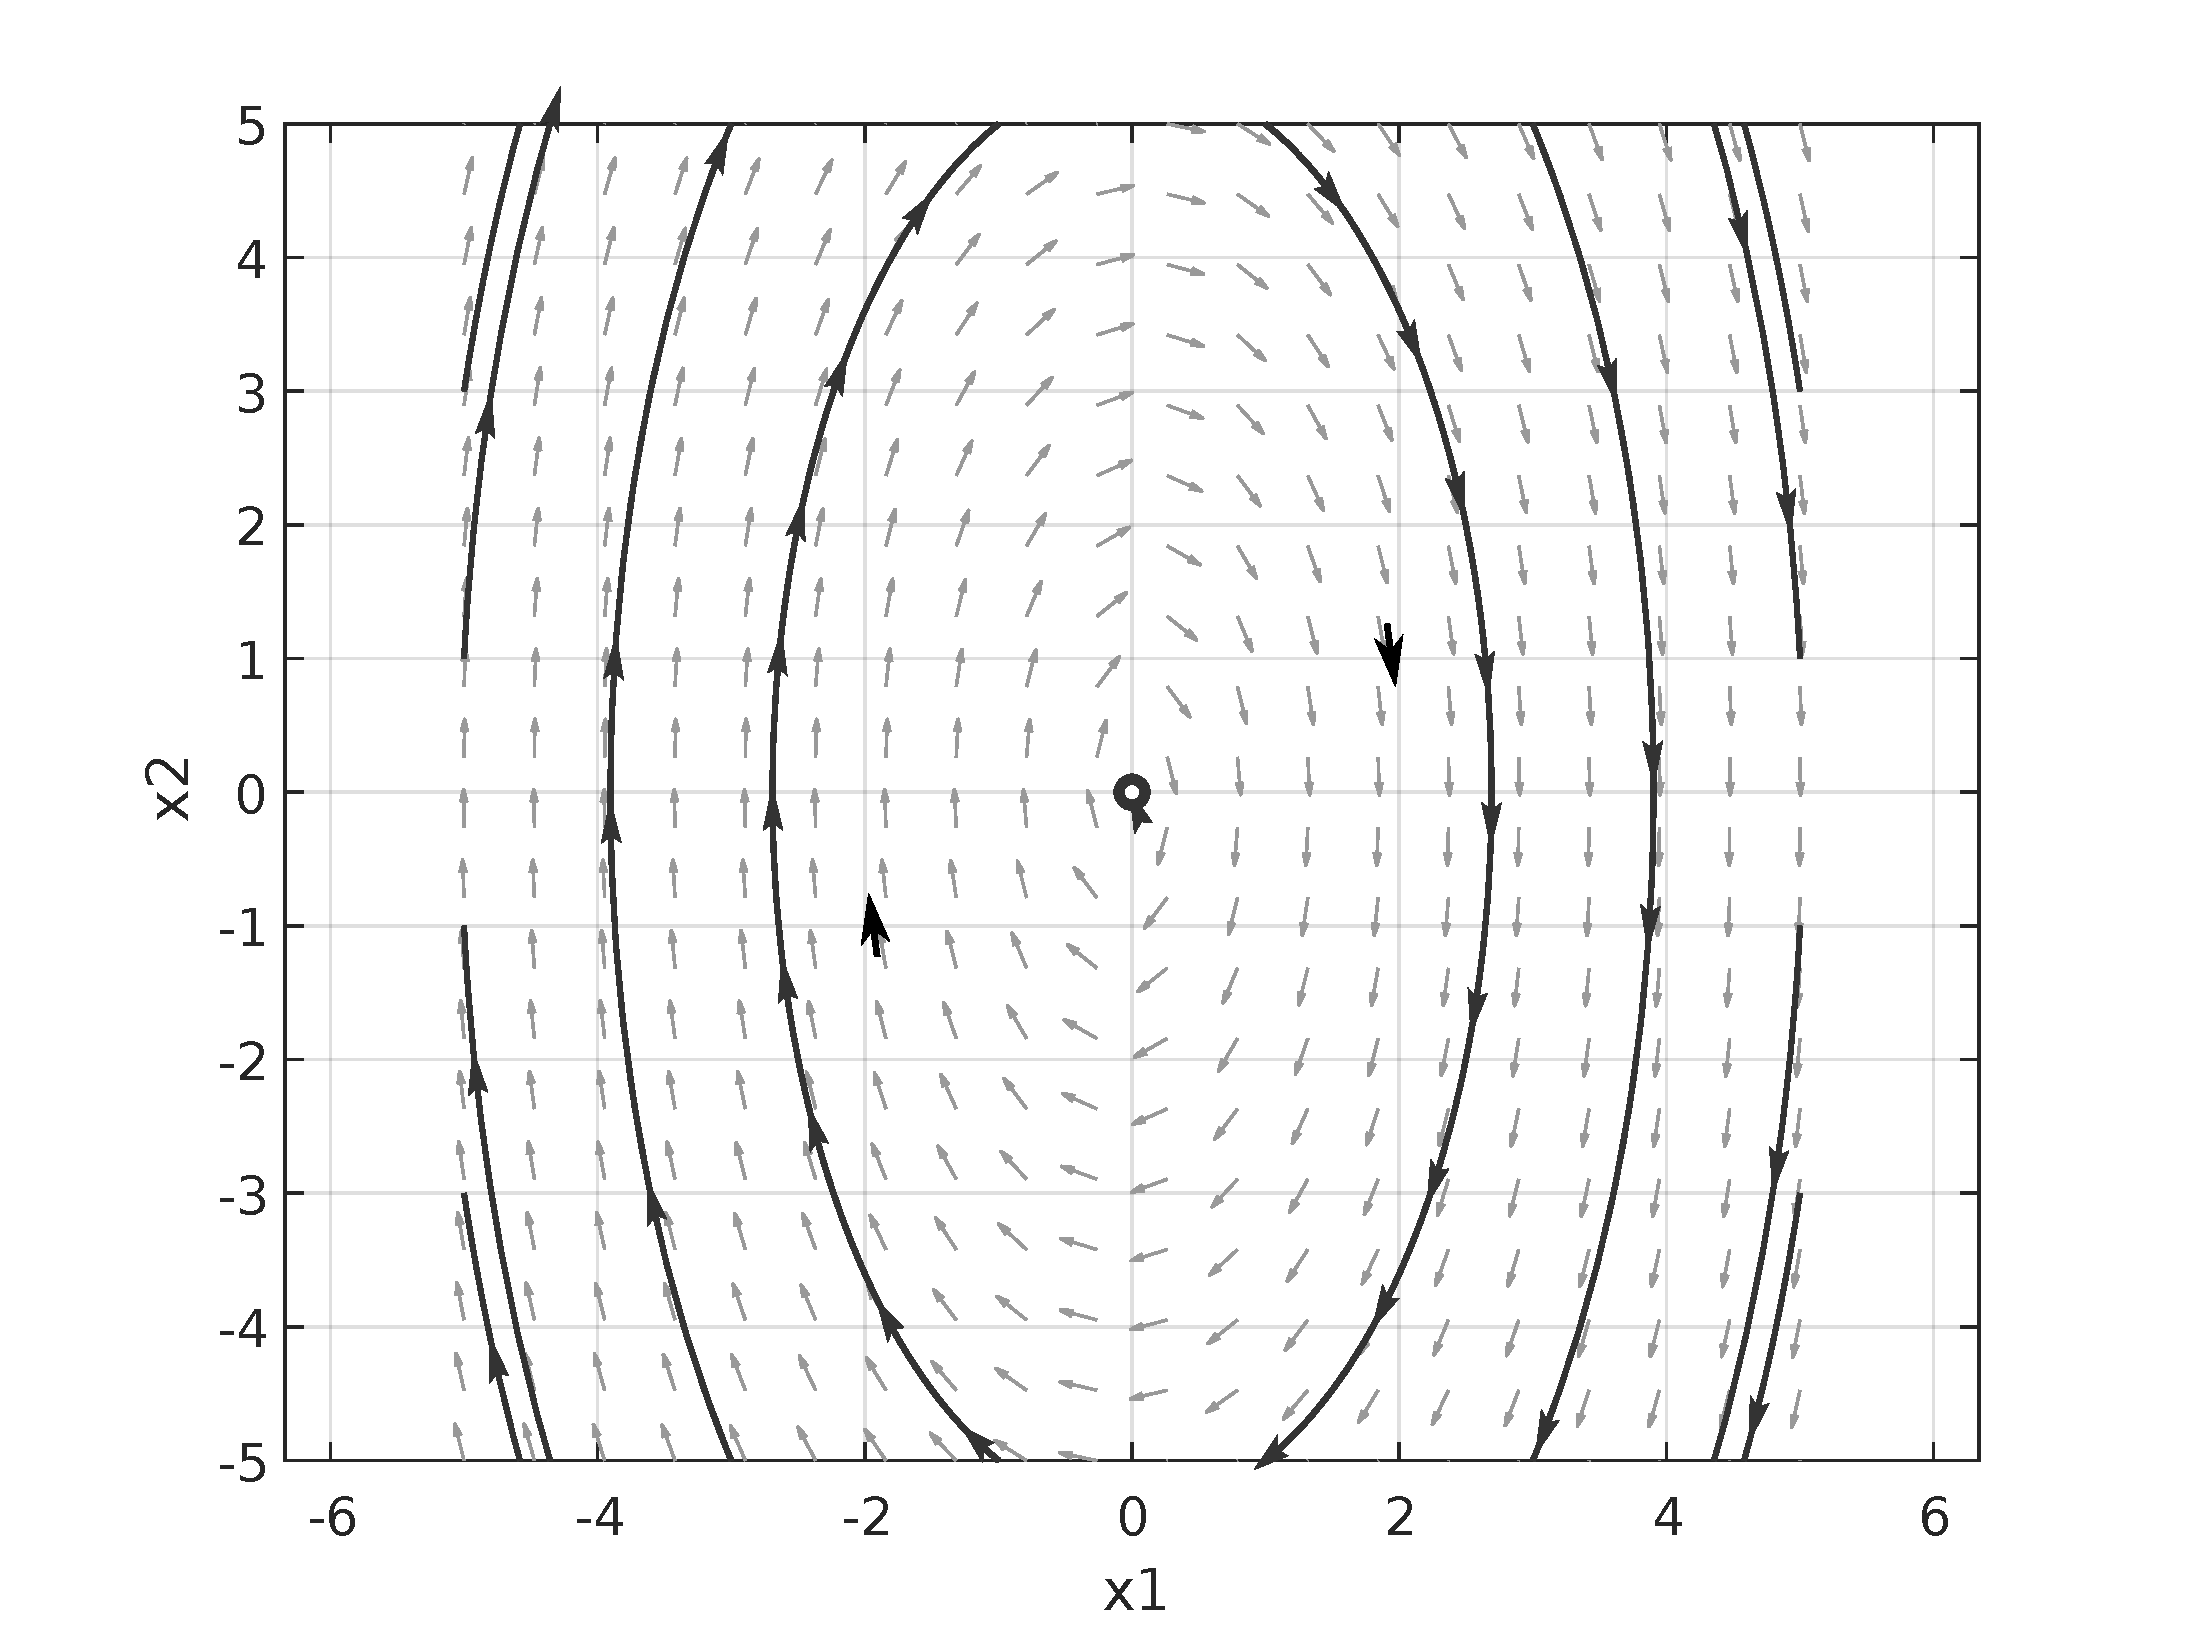
\includegraphics[width=0.3\linewidth]{fig/PureImaginaryPhasePlaneStabCircle.pdf}
    \caption{Portret fazowy rozważanego układu.}
    \label{fig:example_oscillator}
\end{figure}
Dobierzmy sobie przykładowy promień $\epsilon$, który zdefiniuje nam pomarańczową kulę.
\begin{figure}[H]
    \centering
    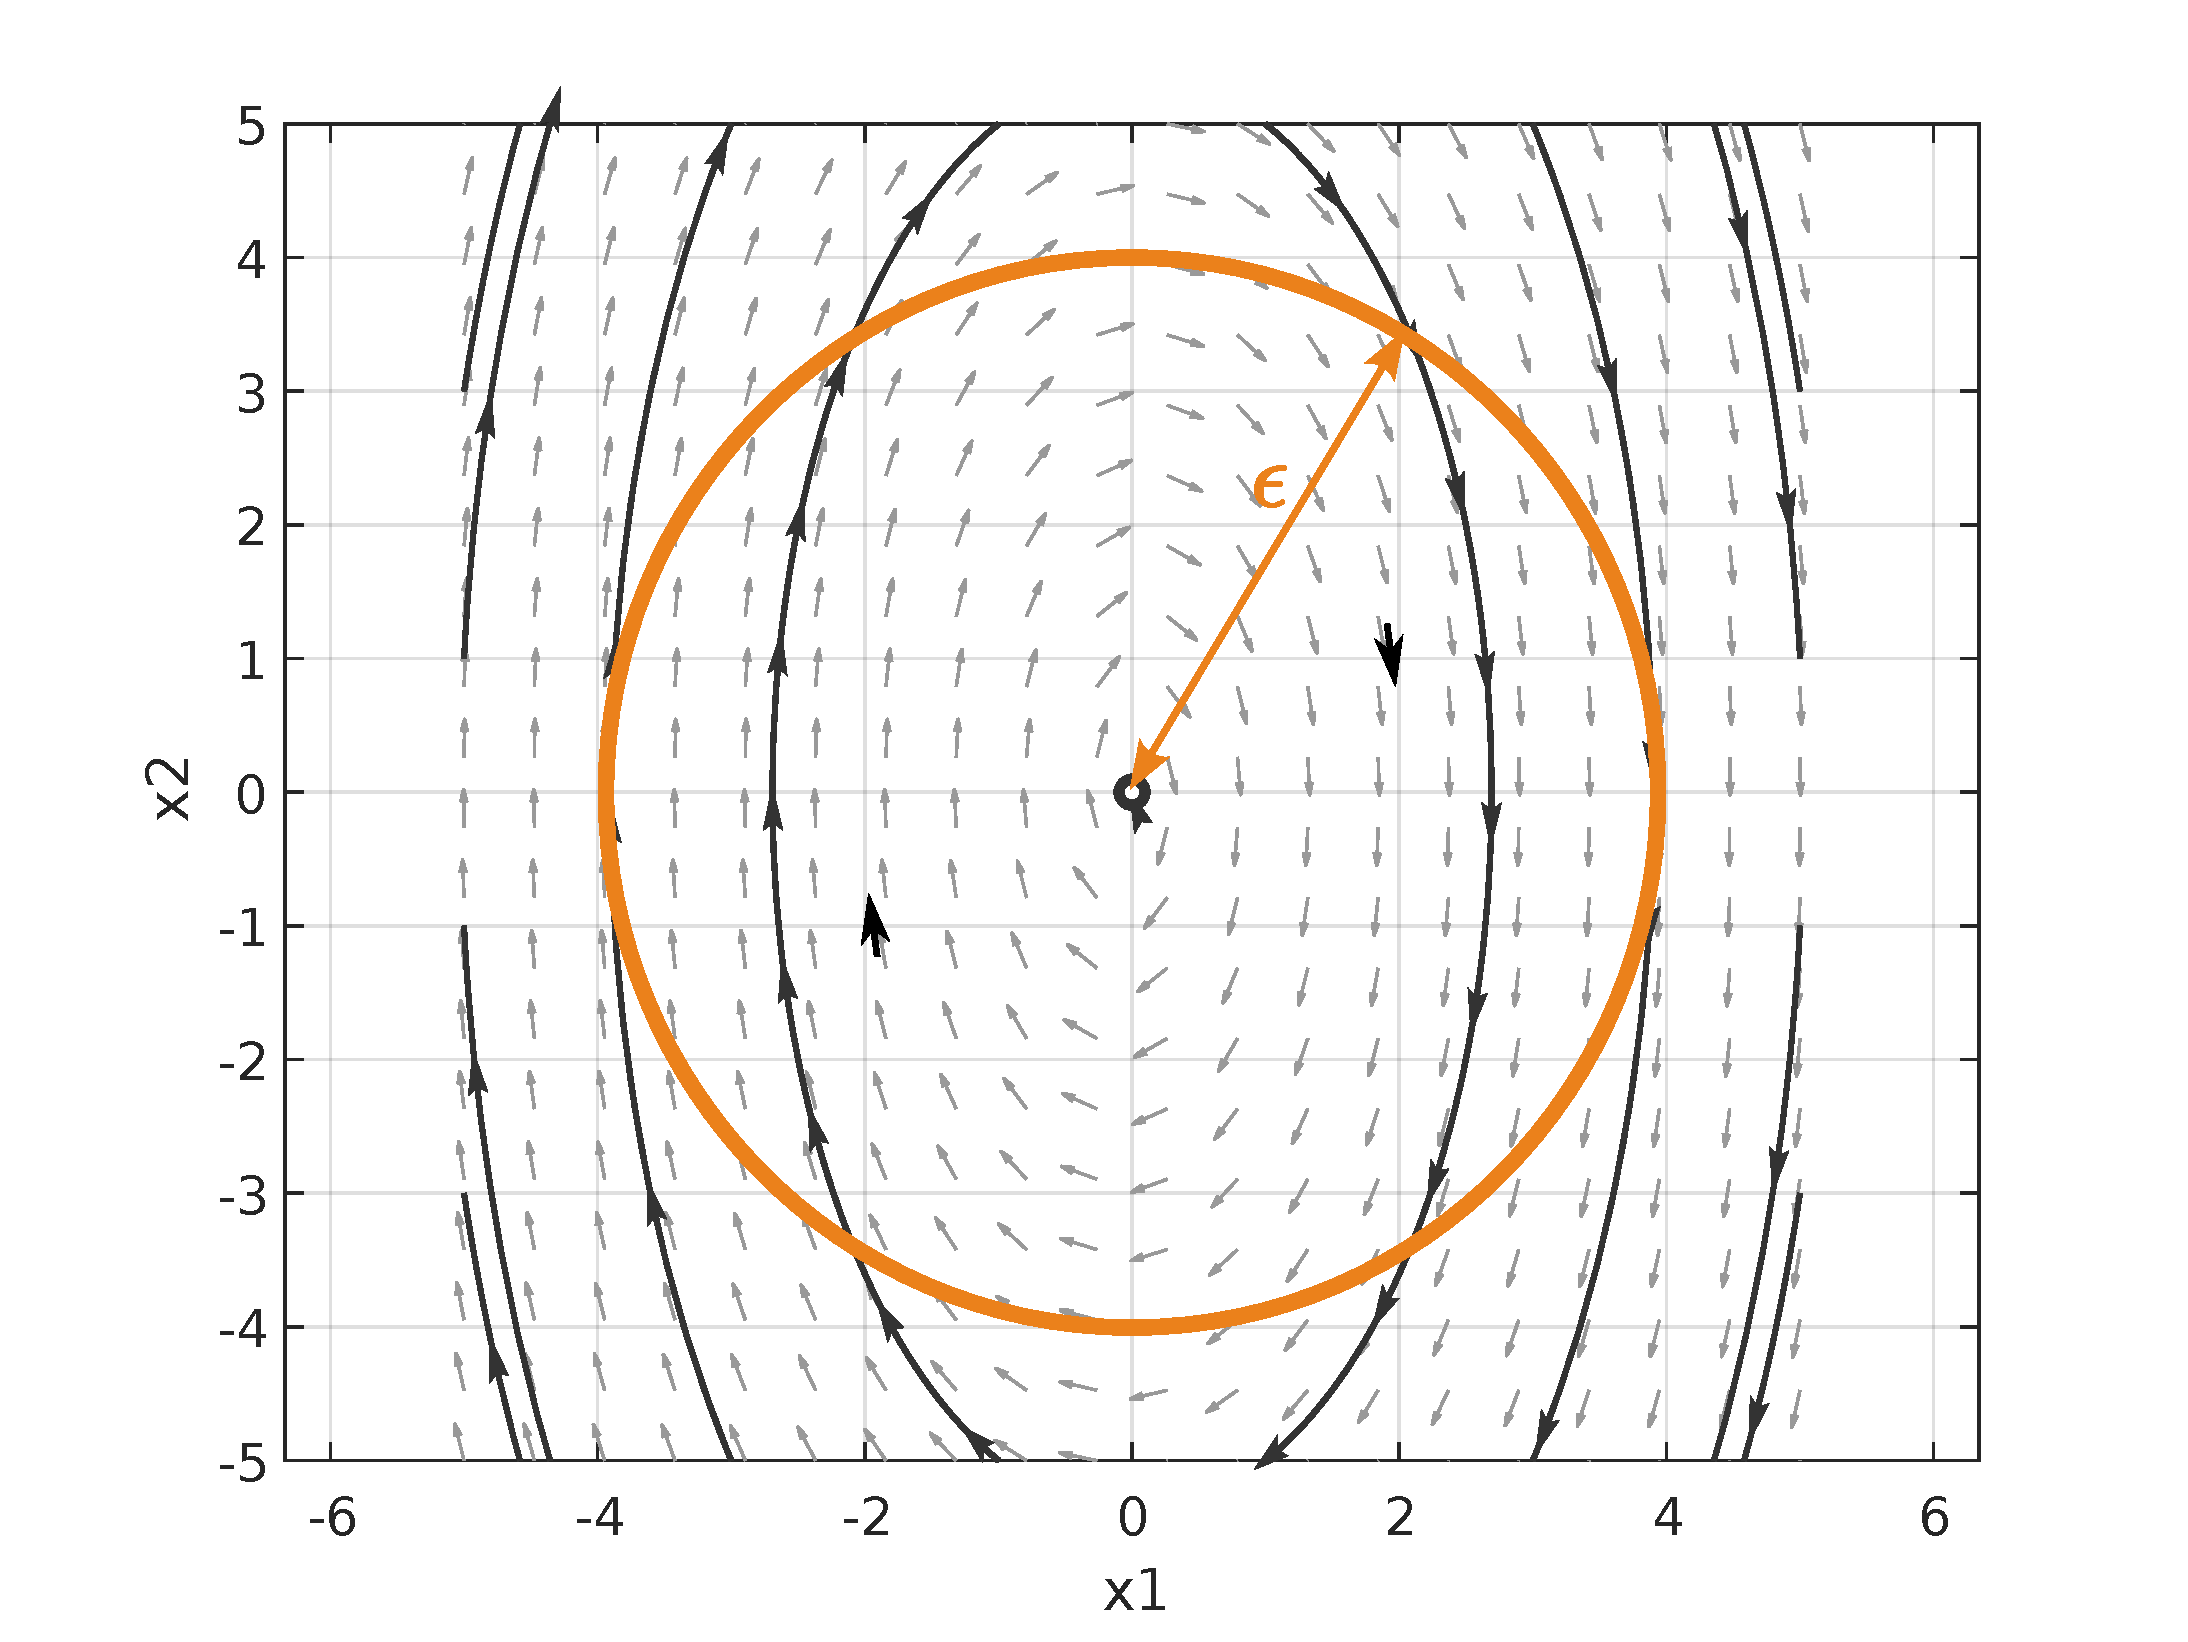
\includegraphics[width=0.3\linewidth]{fig/PureImaginaryPhasePlaneStabCircleStep1.pdf}
    \caption{Promień $\epsilon$ definiuje obszar, w którym chcemy utrzymać stan $x$.}
    \label{fig:example_oscillator_epsilon}
\end{figure}
Dla tego $\epsilon$, jesteśmy w stanie zidentyfikować promień zielonej kuli $\delta_{\epsilon}$, tak by stan nigdy nie wydostał się poza pomarańczową kulę.
\begin{figure}[H]
    \centering
    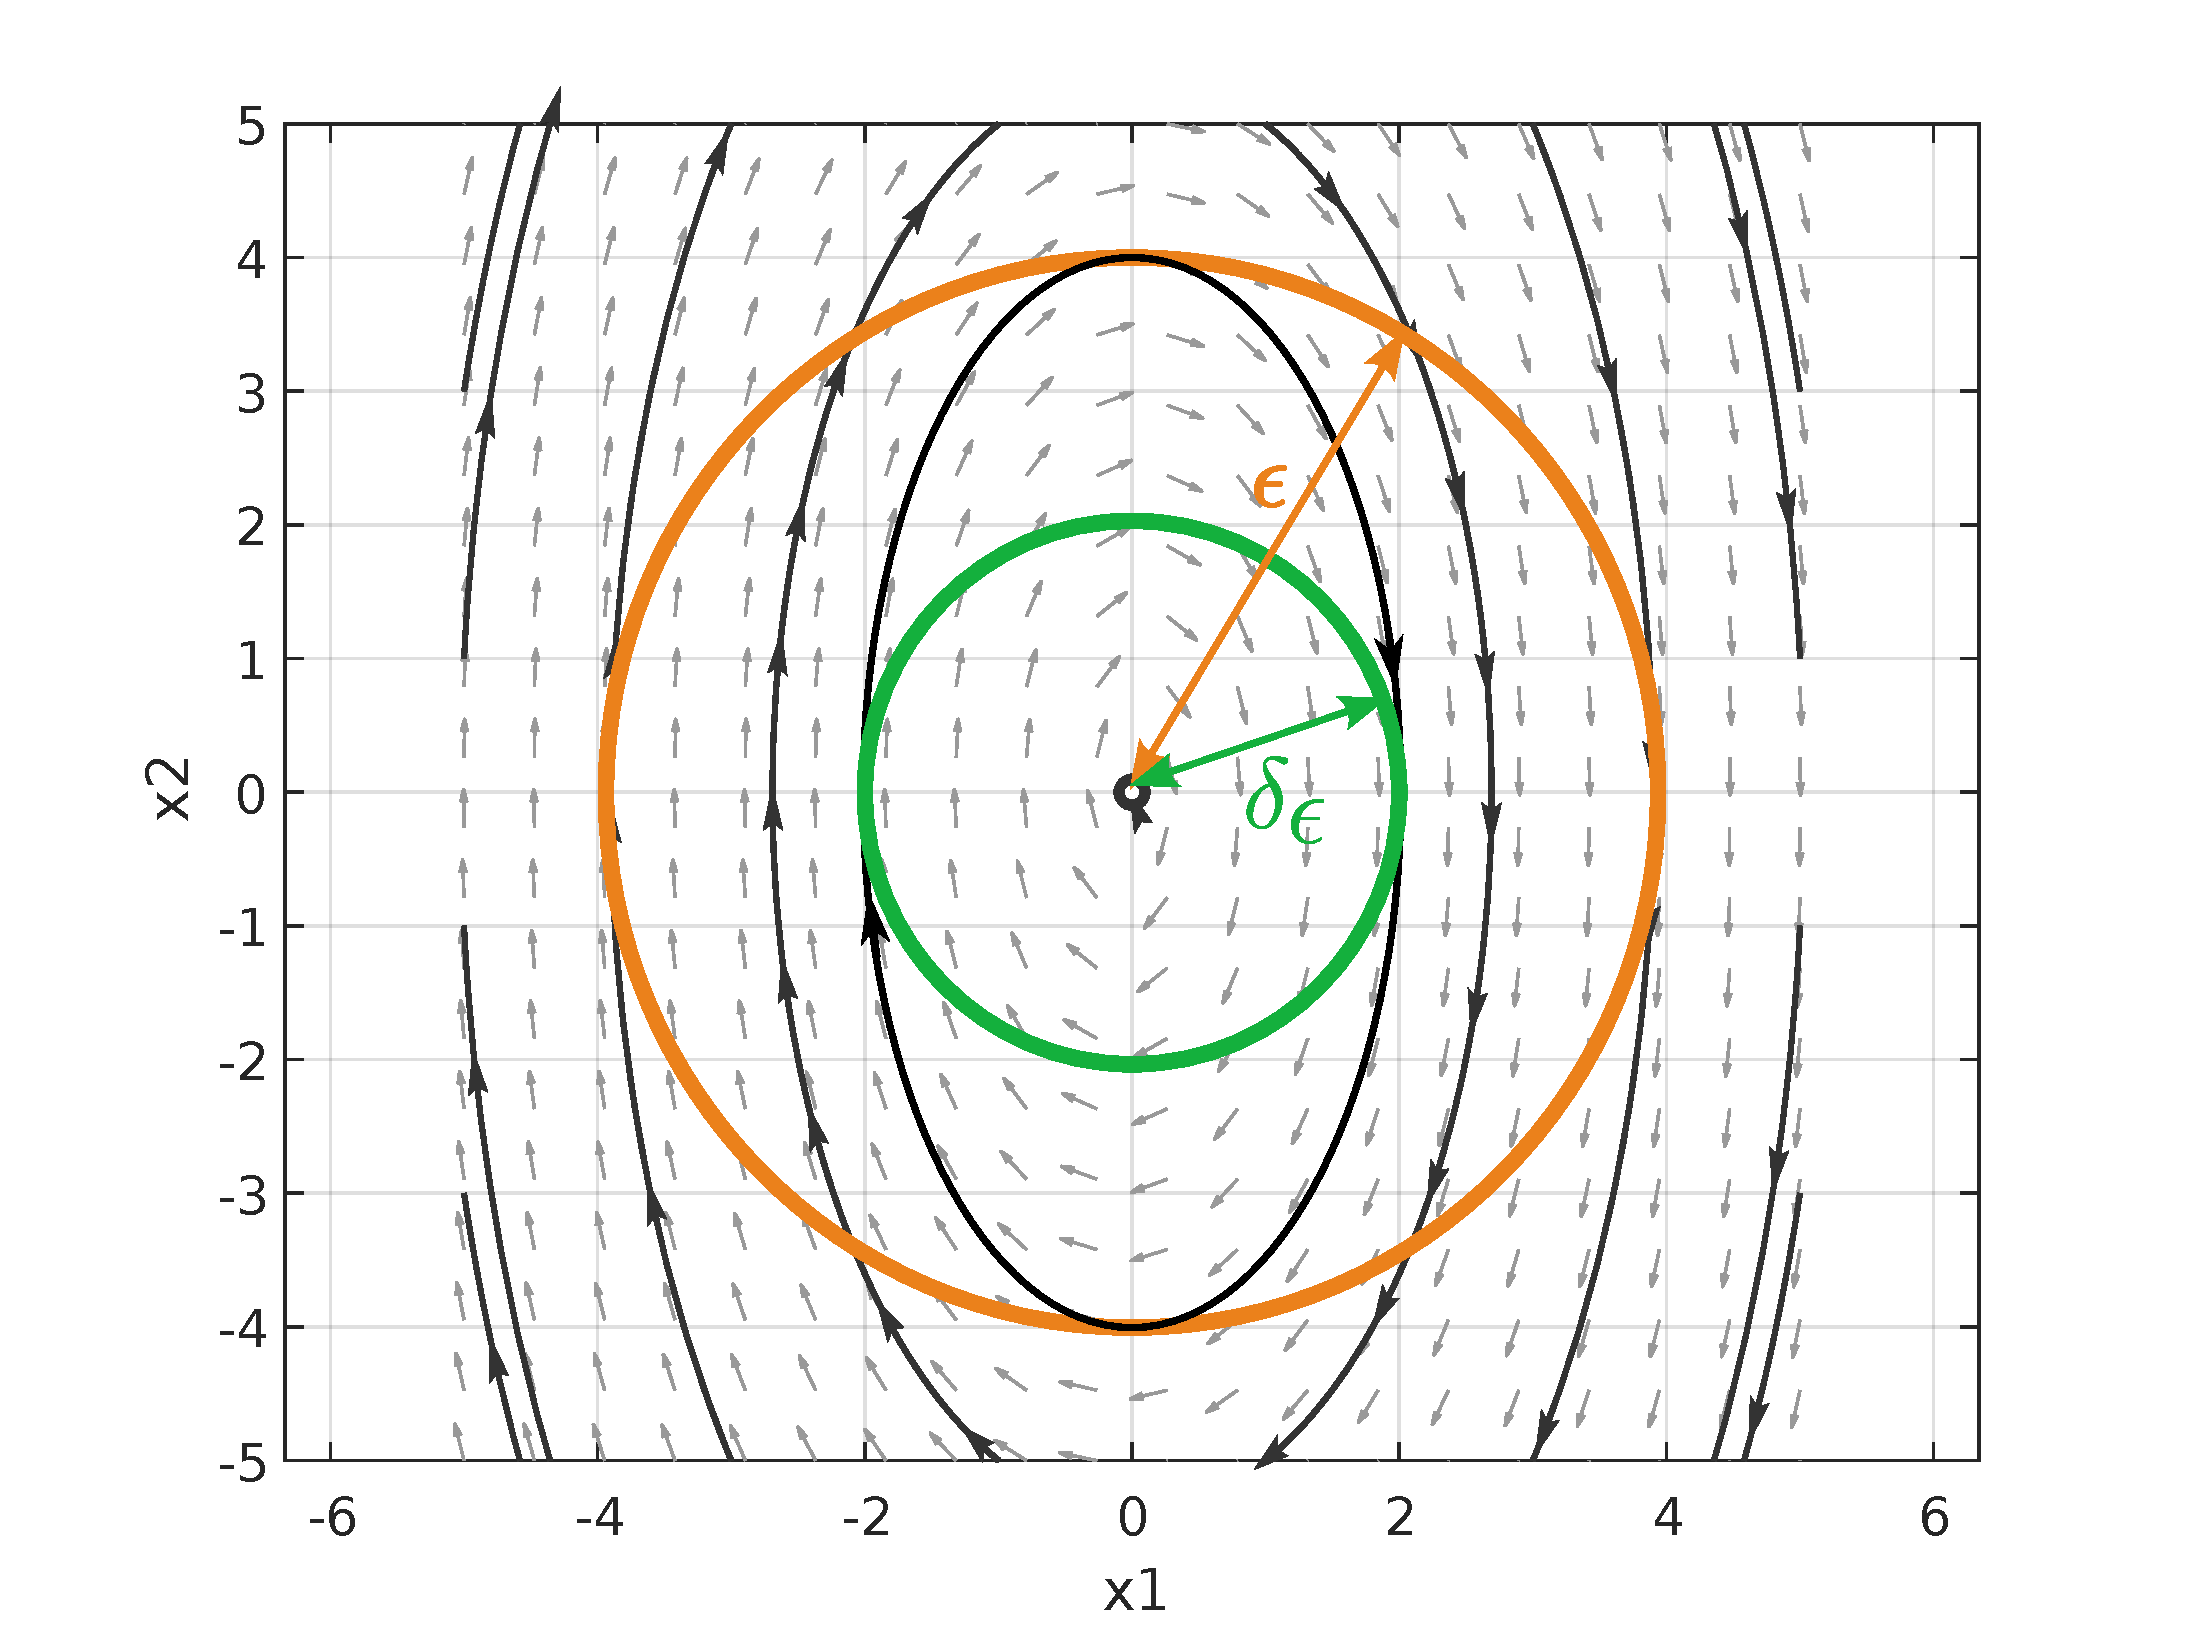
\includegraphics[width=0.3\linewidth]{fig/PureImaginaryPhasePlaneStabCircleAnalysis.pdf}
    \caption{Znalezienie adekwatnego $\delta{\epsilon}$.}
    \label{fig:example_oscillator_delta}
\end{figure}
Ponieważ (w przypadku tego układu) dla jakiejkolwiek pomarańczowej kuli możemy znaleźć adekwatną zieloną kulę, układ ten jest \textbf{stabilny} w sensie Lapunowa. Nie jest on jednak asymptotycznie stabilny.
\end{tcolorbox}


\textbf{Definicja 8}
Punkt równowagi $x_{e}$  układu (\ref{eq:sys}) nazywamy \textbf{stabilnym wykładniczo}, jeśli istnieje $\alpha > 0$ taka, że dla dowolnego $\epsilon > 0$ istnieje $\delta > 0$ takie, że dla dowolnego $t\geq t_{0}$:
\begin{equation}\label{eq:asw}
    \lVert x_{e} - x_{0} \rVert < \delta_{\epsilon}(t_{0}) \implies \lVert x_{e} - x(t;t_{0},x_{0}) \rVert \leq \epsilon e^{-\alpha(t-t_{0})}.
\end{equation}

\textbf{Definicja 9}
Zbiór wszystkich takich punktów $x_{0}$ w przestrzeni stanów, dla których $\lim_{t\rightarrow\infty}\lVert x_{e} - x(t;t_{0},x_{0}) \rVert = 0$ dla pewnego $t_{0} \geq 0$ nazywamy \textbf{zbiorem przyciągania} (\textbf{obszarem atrakcji}) punktu równowagi $x_{e}$.

\textbf{Definicja 10}
Jeżeli punkt równowagi $x_{e}$ jest asymptotycznie stabilny, a jego obszar atrakcji rozciąga się na całą przestrzeń stanów, to punkt równowagi nazywamy \textbf{globalnie asymptotycznie stabilnym}.

\begin{tcolorbox}[colback=green!5, colframe=green!75!black, title=Przykład]
Rozważmy układ opisany układem równań (\ref{eq:przyklad_zbiezny_niestabilny}).
\begin{equation}
    \label{eq:przyklad_zbiezny_niestabilny}
    \left\{
    \begin{array}{l}
         \dot{x}_{1} = \frac{x_{1}^{2}(x_{2}-x_{1}) + x_{2}^{5}}{\left( x_{1}^{2} + x_{2}^{2} \right) \left( 1 + \left( x_{1}^{2} + x_{2}^{2} \right)^{2} \right)}\\
         \dot{x}_{2} = \frac{x_{2}^{2}(x_{2}-2x_{1})}{\left( x_{1}^{2} + x_{2}^{2} \right) \left( 1 + \left( x_{1}^{2} + x_{2}^{2} \right)^{2} \right)}
    \end{array}
    \right\}.
\end{equation}
Układ ten ma jeden punkt równowagi w początku układu współrzędnych, a jego obszarem atrakcji jest cała płaszczyzna $\mathbb{R}^{2}$, lecz nie jest on stabilny. Ponieważ nie można dobrać takiego $\delta$, aby implikacja (\ref{eq:lyap_def}) była spełniona.
Kilka jego przykładowych trajektorii okazano na rysunku (\ref{fig:example_unstable}).
\begin{figure}[H]
    \centering
    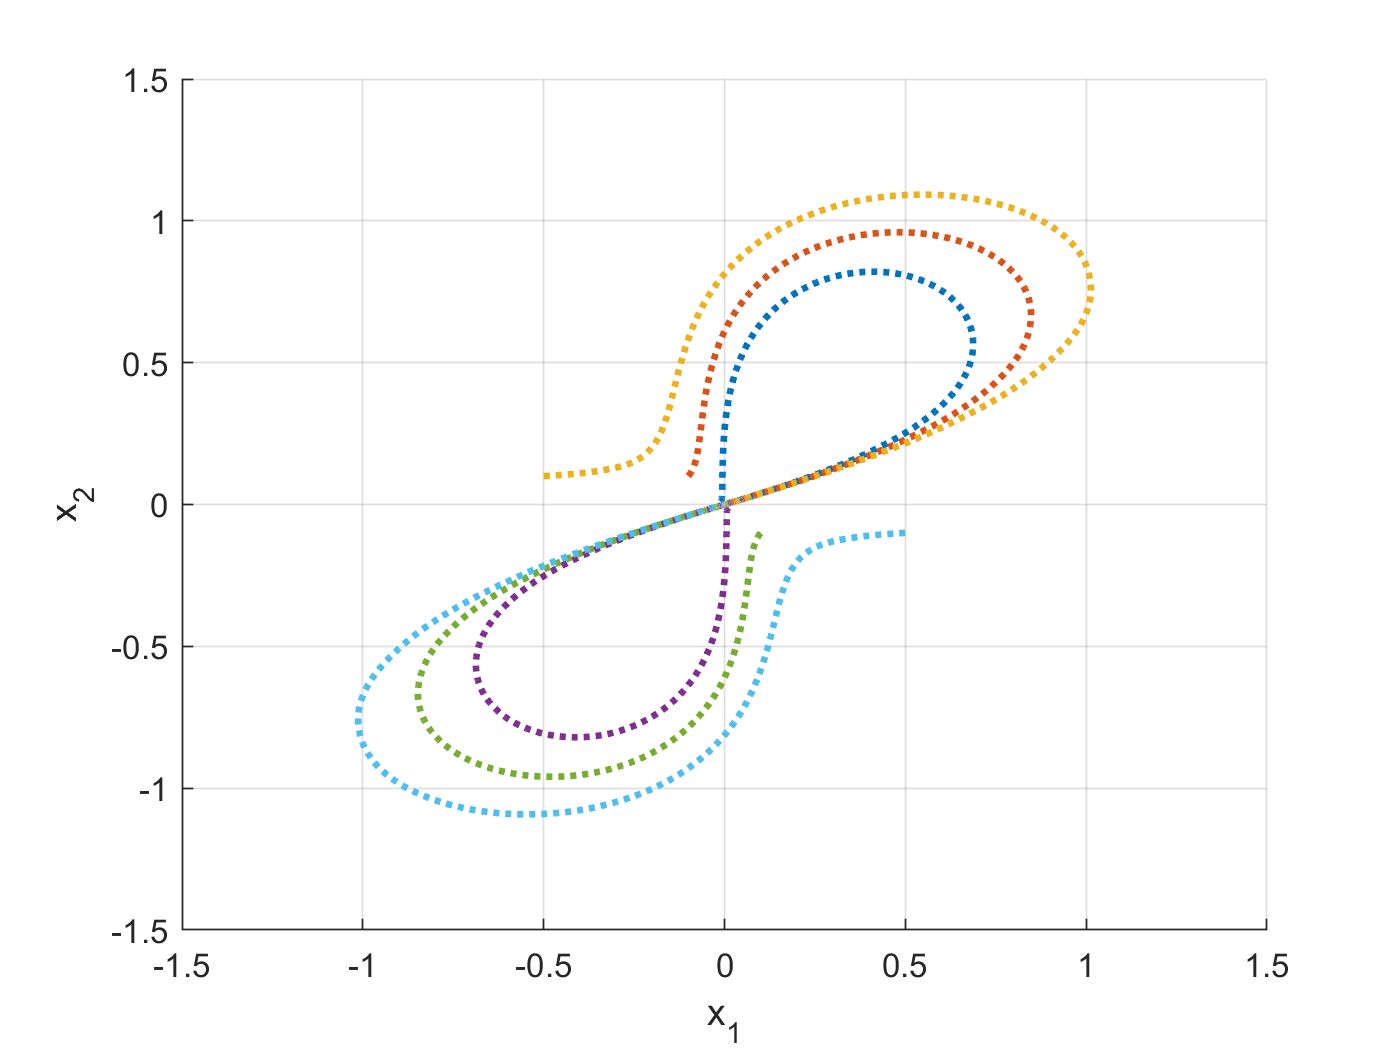
\includegraphics[width=0.5\linewidth]{fig/przyklad_atr_stab.PNG}
    \caption{Przykładowe trajektorie dla układu (\ref{eq:przyklad_zbiezny_niestabilny}).}
    \label{fig:example_unstable}
\end{figure}
\end{tcolorbox}

\newpage
\subsection{Twierdzenie Lapunowa}
\textbf{Definicja 11}
Funkcja $V: D \rightarrow \mathbb{R}$ jest nazywana:
\begin{itemize}
    \item dodatnio określoną, jeśli $V(0) = 0$ i $\forall_{x\neq 0}V(x) > 0$,
    \item dodatnio półokreśloną, jeśli $V(0) = 0$ i $\forall_{x\neq 0}V(x) \geq 0$,
    \item ujemnie określoną (półokreśloną), jeśli $-V(x)$ jest dodatnio określona (półokreślona).
\end{itemize}

Dalsze definicje i twierdzenia odnoszą się do systemów stacjonarnych:
\begin{equation}\label{eq:sys_stac}
    \dot{x} = f(x).
\end{equation}
\textbf{Definicja 12}
Funkcja $\dot{V}: D \rightarrow \mathbb{R}$ oraz 
$$
    \dot{V}(x)=\nabla V(x)f(x) = \mathcal{L}_{f}V(x) = \begin{bmatrix} \frac{\partial V}{\partial x_{1}} & \frac{\partial V}{\partial x_{2}} & \cdots & \frac{\partial V}{\partial x_{n}} \end{bmatrix}
    \begin{bmatrix} f_{1}(x) \\ f_{2}(x) \\ \vdots \\ f_{n}(x) \end{bmatrix}
$$
nazywana jest pochodną wzdłuż trajektorii systemu (\ref{eq:sys_stac}) lub pochodną systemową funkcji $V$ albo pochodną Lie'go wzdłuż pola wektorowego $f$ i oznacza $\mathcal{L}_{f}V(x)$.

\textbf{Twierdzenie 1 (Lapunowa)}
Jeżeli istnieje funkcja $V: D \rightarrow \mathbb{R}$, która jest:
\begin{itemize}
    \item różniczkowalna w sposób ciągły,
    \item dodatnio określona w $D$,
    \item jej pochodna systemowa $\dot{V}:D\rightarrow \mathbb{R}$ jest ujemnie półokreślona w $D$
\end{itemize}
to punkt równowagi $x_{e} = 0$ układu (\ref{eq:sys_stac}) jest stabilny.
A jeśli pochodna systemowa jest ujemnie określona w $D$, to punkt równowagi $x_{e} = 0$ układu (\ref{eq:sys_stac}) jest asymptotycznie stabilny.

\begin{tcolorbox}[colback=blue!5, colframe=blue!75!black, title=Ważne]
Twierdzenie Lapunowa dostarcza warunek konieczny i wystarczający stabilności punktu równowagi, jednak nie dostarcza żadnej informacji o tym, jak odnaleźć funkcję $V(x)$. Odnalezienie tej funkcji jest zasadniczą trudnością w badaniu stabilności.
W punkcie \ref{sec:dobor_funkcji} podano kilka metod poszukiwania funkcji Lapunowa.
\end{tcolorbox}

\textbf{\textit{Dowód:}}
\textit{Stabilność:}
Zgodnie z \textit{definicją 4 }weźmy liczbę $\epsilon > 0$.
Załóżmy, że kula o promieniu $\epsilon$ zawiera się w~zbiorze $D$:
$$
    K_{\epsilon} = \left\{ x\in \mathbb{R}^{n}: \lVert x \rVert \leq \epsilon \right\} \subset D.
$$
Niech:
$$
    \alpha = \min_{\lVert x \rVert = \epsilon }V(x).
$$
Weźmy liczbę $\beta$, taką że $0 < \beta < \alpha$ i oznaczmy zbiór:
$$
    \Omega_{\beta} = \left\{ x \in K_{\epsilon}: V(x) < \beta \right\}.
$$
Zachodzi więc $\Omega_{\beta} \subset K_{\epsilon}$.
Rozważając dowolną trajektorię $x(t) = x(t; t_{0}, x_{0})$ układu (\ref{eq:sys_stac}), taką że $x_{0} \in \Omega_{\beta}$.
Wzdłuż tej trajektorii mamy $\dot{V}(x) \leq 0$, więc $V(x(t)) \leq V(x_{0}) \leq \beta$, czyli cała trajektoria $x(t)$ pozostanie w zbiorze $\Omega_{\beta} \subset K_{\beta}$ dla dowolnego $t$.
Ponadto z ciągłości funkcji $V(x)$ wynika, że istnieje $\delta > 0$ taka, że:
$$
    \lVert x \rVert < \delta \implies V(x) < \beta
$$
czyli zachodzi $K_{\delta} = \left\{ x \in \mathbb{R}^{n}| \Vert x \rVert < \delta \right\} \subset \Omega_{\beta} \subset K_{\beta}$. Tak więc, z takim wyborem $\delta$ implikacja
$$
    \lVert x \rVert < \delta \implies \lVert x \rVert < \epsilon
$$
jest prawdziwa i zgodnie z \textit{definicją 4} $x_{e} = 0$ jest stabilny w sensie Lapunowa.

\textit{Asymptotyczna stabilność:}
Jeżeli pochodna systemowa $\dot{V}:D \rightarrow \mathbb{R}$ jest ujemnie określona w $D$, to wzdłuż trajektorii $x(t) = x(t; t_{0}, x_{0})$ układ (\ref{eq:sys_stac}) funkcja $V(x)$ jest ściśle malejąca i ograniczona od dołu przez 0, więc zbiega do nieujemnej granicy $c$:
$$
    \lim_{t \rightarrow \infty} V(x(t)) = c \geq 0.
$$
Jeśli przypuścimy, że $c > 0$, to oznaczałoby to, że cała trajektoria $x(t)$ pozostaje na zewnątrz zbioru $\Omega_{c} = \left\{ x \in K_{\epsilon}: V(x) \leq c \right\}$, a tym samym na zewnątrz dowolnej kuli $K_{r} = \left\{ x \in \mathbb{R}^{n}: \Vert x \rVert \leq r \right\}$ zawartej w $\Omega_{c}$.
Wtedy wzdłuż trajektorii $x(t)$
$$
    \dot{V}(x) \leq \max_{r \leq \lVert x \rVert \leq \epsilon} \dot{V}(x) = -v < 0
$$
czyli
$$
    V(x(t)) = V(x(t_{0})) + \int_{t_{0}}^{t}{\dot{V}(x(\tau))d\tau} \leq V(x(t_{0})) - v(t - t_{0}).
$$
Dla dostatecznie dużego $t$ funkcja $V(x(t))$ przyjmowałaby więc wartości ujemne, co jest sprzeczne z założeniami co do funkcji $V(x)$.
Musi więc zachodzić:
$$
    \lim_{t \rightarrow \infty}V(x(t)) = 0
$$
co pociąga za sobą:
$$
    \lim_{t \rightarrow\infty} x(t) = 0
$$
i udowadnia asymptotyczną stabilność.
\begin{figure}[H]
    \centering
    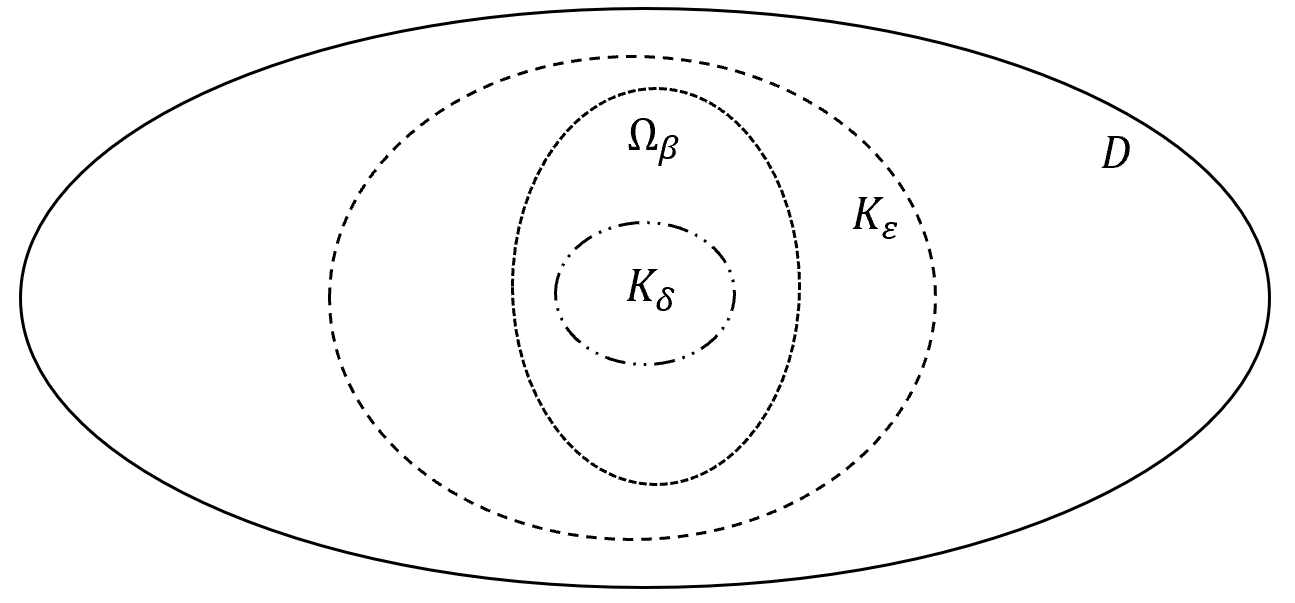
\includegraphics[width=0.5\linewidth]{fig/lap_dowod_zbiory.PNG}
    \caption{Zbiory definiowane w dowodzie twierdzenia Lapunowa o stabilności.}
    \label{fig:enter-label}
\end{figure}

\textbf{Definicja 13}
Funkcja $V:D\rightarrow\mathbb{R}$ spełniająca założenia twierdzenia Lapunowa jest nazywana funkcją Lapunowa.

\begin{figure}[H]
    \centering
    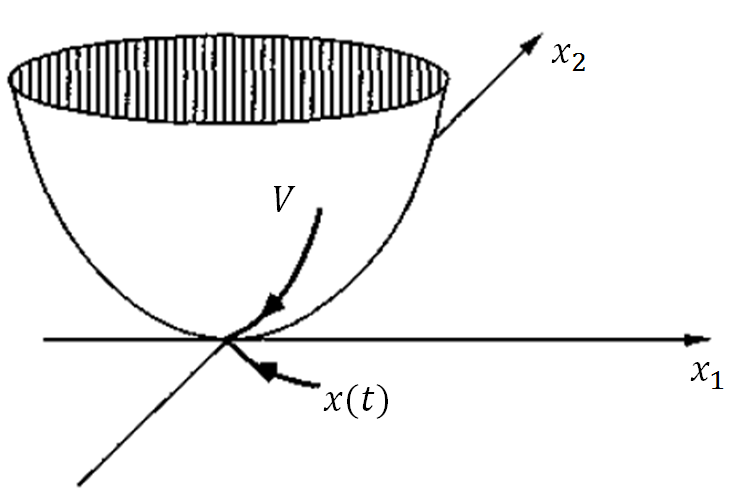
\includegraphics[width=0.5\linewidth]{fig/funkcja_lapunowa.PNG}
    \caption{Graficzna interpretacja funkcji Lapunowa dla $n=2$.}
    \label{fig:lapunowa_interpretacja2}
\end{figure}

\textbf{Twierdzenie 2 (Lapunowa o niestabilności)}
Jeżeli istnieje funkcja $V:D\rightarrow \mathbb{R}$ różniczkowalna w sposób ciągły, dodatnio określona w pewnym otoczeniu punktu równowagi $x_{e} = 0$ i taka, że jej pochodna systemowa $\dot{V}:D\rightarrow\mathbb{R}$ jest dodatnio określona w pewnym zbiorze $G = \left\{ x \in K_{\epsilon} : V(x) > 0 \right\}$, gdzie $K_{\epsilon} = \left\{ x \in \mathbb{R}^{n}: \lVert x \rVert \leq \epsilon \right\} \subset D$, to punkt równowagi $x_{e} = 0$ jest niestabilny.

\begin{tcolorbox}[colback=blue!5, colframe=blue!75!black, title=Ważne]
\textbf{Funkcje Lapunowa dla układów liniowych}
W przypadku układów liniowych, które mają ściśle określoną strukturę:
\begin{equation}\label{eq:sys_lin}
    \dot{x} = Ax
\end{equation}
można wykazać, że jeśli istnieje dodatnio określona i symetryczna macierz $P \in \mathbb{R}^{n}$, która spełnia tzw. równanie Lapunowa:
\begin{equation}\label{eq:rownanie_lapunowa}
    A^{T}P + PA = -Q
\end{equation}
gdzie: $Q=Q^{T} > 0$,
to dla układu (\ref{eq:sys_lin}) funkcja Lapunowa istnieje i ma postać:
\begin{equation}
    V(x) = x^{T}Px.
\end{equation}
A jej pochodna systemowa ma postać:
\begin{equation}\label{eq:lin_lap_div}
    \dot{V}(x) = \dot{x}^{T}Px + xP\dot{x} = x^{T}(A^{T}P + PA)x = -x^{T}Qx
\end{equation}
Jest to równoważne z położeniem widma macierzy $A$ w lewej półpłaszczyźnie
zespolonej.
\end{tcolorbox}

\textbf{Twierdzenie 3 (pośrednia metoda Lapunowa)}
Jeżeli badany układ \ref{eq:sys_stac} jest tzw. systemem \textit{słabo-nieliniowym}, tzn. można go zapisać w postaci:
\begin{equation}\label{eq:sys_slabo_niel}
    \dot{x} = Ax + r(x)
\end{equation}
gdzie:
\begin{itemize}
    \item $A \in \mathbb{R}^{n}$,
    \item $r(x): \mathbb{R}^{n} \rightarrow \mathbb{R}^{n}$ jest różniczkowalną, lokalnie lipschitzowską funkcją, która ponadto spełnia warunek:
    \begin{equation}\label{eq:warunek_slabo_niel}
        \lim_{\lVert x \rVert \rightarrow 0} \frac{\lVert r(x) \rVert}{\lVert x \rVert} = 0
    \end{equation}
\end{itemize}
to stabilność punktu równowagi może być analizowana w oparciu o przybliżenie liniowe, zaniedbujące składnik $r(x)$, to znaczy:
$$  
    \dot{x} = Ax.
$$
Wówczas stabilność punktu równowagi zależy od widma macierzy $A$ (jej wartości własnych) w następujący sposób:
\begin{enumerate}
    \item Jeżeli wszystkie wartości własne macierzy $A$ spełniają warunek $Re(\lambda) < 0$, czyli leżą w lewej półpłaszczyźnie zespolonej,  to punkt równowagi jest asymptotycznie stabilny.
    \item Jeżeli którakolwiek z wartości własnych macierzy $A$ leży w prawej półpłaszczyźnie zespolonej, to punkt równowagi jest niestabilny.
    \item Jeżeli wartości własne macierzy $A$ leżą w lewej półpłaszczyźnie zespolonej i choć jeden na osi urojonych, to nie można wnioskować o stabilności punktu równowagi na podstawie przybliżenia liniowego.
\end{enumerate}

\begin{tcolorbox}[colback=orange!5, colframe=orange!75!black, title=Uwaga]
Możliwość zastosowania analizy układu zlinearyzowanego wynika z~twierdzenia
Hartmana-Grobmana, które mówi, że w~otoczeniu punktu równowagi układ nieliniowy
jest topologicznie równoważny z~jego przybliżeniem liniowym (możemy znaleźć lokalny
homeomorfizm z~układu nieliniowego w~liniowy), o~ile wszystkie
wartości własne macierzy $A$ mają część rzeczywistą różną od zera.
Oznacza to, że w~takim przypadku zachowanie układu nieliniowego w~otoczeniu
punktu równowagi jest podobne do zachowania układu liniowego. 
\end{tcolorbox}

\begin{tcolorbox}[colback=green!5, colframe=green!75!black, title=Przykład]
Rozpatrzmy prosty układ pierwszego rzędu:
$$
    \dot{x} = ax + bx^3.
$$
Jego przybliżenie liniowe ma postać:
$$
    \dot{x} = ax
$$
Ponadto $r(x) = bx^3$ jest ciągła, lipschitzowska i spełnia warunek
$$
    \lim_{\lVert x \rVert \rightarrow 0} \frac{\lVert bx^3 \rVert}{\lVert x \rVert} = \lim_{\lVert x \rVert \rightarrow 0} |b| \lVert x^2 \rVert = 0.
$$
Mamy zatem 3 przypadki:
\begin{itemize}
    \item $a<0$ - wówczas układ stabilny,
    \item $a>0$ - wówczas układ niestabilny,
    \item $a=0$ - wtedy o stabilności decyduje $r(x) = bx^3$ - jeśli $b<0$ to stabilny, a jeśli $b>0$ to niestabilny.
\end{itemize}
Łatwo jest to zweryfikować bezpośrednią metodą Lapunowa, przyjmując funkcję Lapunowa $V(x) = \frac{1}{2}x^{2}$.
\end{tcolorbox}

\begin{tcolorbox}[colback=orange!5, colframe=orange!75!black, title=Uwaga]
    Skoro z twierdzenia Hartmana-Grobmana wynika, że w~otoczeniu punktu
    równowagi układ nieliniowy jest topologicznie równoważny z~jego
    przybliżeniem liniowym, to dlaczego by nie znaleźć funkcji, która
    przekształca go w układ liniowy i~nie zastosować do niego bezpośredniej
    metody Lapunowa?
    Metoda ta nazywana jest linearyzującym sprężeniem zwrotnym (ang. feedback
    linearization).
\end{tcolorbox} 

    %===========================================================
    \subsection{Przykłady}
        %-------------------------------------------------------
        \subsubsection{Przykład 1}
        Zbadać stabilność punktów równowagi układu równań różniczkowych:
        \begin{equation}\label{eq:example_11_sys_transformed}
            \left\{
            \begin{array}{l}
                 \dot{x}_{1} = x_{1}^{2} - x_{2}\\
                 \dot{x}_{2} = x_{1} - x_{2}
            \end{array}
            \right\}.
        \end{equation}
        W celu wyznaczenia punktów równowagi przyrównujemy prawą stronę równania (\ref{eq:example_11_sys_transformed}) do zera i otrzymujemy dwa punkty równowagi:
        \begin{enumerate}
            \item $x_{e}^{1} = \begin{bmatrix} 0 & 0 \end{bmatrix}^{T}$:
            Badany układ można zapisać w postaci (\ref{eq:sys_slabo_niel}) z \textbf{twierdzenia 2}:
            $$
                \begin{bmatrix} \dot{x}_{1} \\ \dot{x}_{2} \end{bmatrix}
                =
                \begin{bmatrix} 0 & -1 \\ 1 & -1 \end{bmatrix}
                \begin{bmatrix} x_{1} \\ x_{2} \end{bmatrix}
                +
                \begin{bmatrix} x_{1}^{2} \\ 0 \end{bmatrix}
            $$
            gdzie:
            \begin{itemize}
                \item $A = \begin{bmatrix} 0 & -1 \\ 1 & -1 \end{bmatrix}$,
                \item $r(x) = \begin{bmatrix} x_{1}^{2} & 0 \end{bmatrix}^{T}$ i $\lim_{\lVert x \rVert \rightarrow 0}\frac{\lVert r(x) \rVert}{\lVert x \rVert} = \lim_{\lVert x \rVert \rightarrow 0}\frac{x_{1}^{2}}{\lVert x \rVert} = 0$.
            \end{itemize}
            Badamy zatem wartości własne macierzy $A$:
            $$
                \begin{vmatrix} \lambda & 1\\ -1 & \lambda + 1 \end{vmatrix} = \lambda^{2} + \lambda + 1 = 0.
            $$
            Pierwiastki równania mają części rzeczywiste ujemne, zatem $x_{e}^{1}$ jest stabilnym punktem równowagi.
            
            \item $x_{e}^{2} = \begin{bmatrix} 1 & 1 \end{bmatrix}^{T}$: Aby móc zastosować pośrednią metodę Lapunowa przesuwamy punkt równowagi do początku układu współrzędnych: $z_{1} = x_{1} - 1$, $z_{2} = x_{2} - 1$. Wówczas układ (\ref{eq:example_11_sys_transformed}) przybiera formę:
            $$
                \left\{
                \begin{array}{l}
                     \dot{z}_{1} = z_{1}^{2} + 2z_{1} - z_{2}\\
                     \dot{z}_{2} = z_{1} - z_{2}
                \end{array}
                \right\}.
            $$
            Więc badany układ można zapisać w postaci (\ref{eq:sys_slabo_niel}) z \textbf{twierdzenia 2}:
            $$
                \begin{bmatrix} \dot{z}_{1} \\ \dot{z}_{2} \end{bmatrix}
                =
                \begin{bmatrix} 2 & -1 \\ 1 & -1 \end{bmatrix}
                \begin{bmatrix} z_{1} \\ z_{2} \end{bmatrix}
                +
                \begin{bmatrix} z_{1}^{2} \\ 0 \end{bmatrix}
            $$
            gdzie:
            \begin{itemize}
                \item $A = \begin{bmatrix} 2 & -1 \\ 1 & -1 \end{bmatrix}$,
                \item $r(z) = \begin{bmatrix} z_{1}^{2} & 0 \end{bmatrix}^{T}$ i $\lim_{\lVert z \rVert \rightarrow 0}\frac{\lVert r(z) \rVert}{\lVert z \rVert} = \lim_{\lVert z \rVert \rightarrow 0}\frac{z_{1}^{2}}{\lVert z \rVert} = 0$.
            \end{itemize}
            Badamy zatem wartości własne macierzy $A$:
            $$
                \begin{vmatrix} \lambda-2 & 1\\ -1 & \lambda + 1 \end{vmatrix} = \lambda^{2} - \lambda + 1 = 0.
            $$
            Pierwiastki równania mają części rzeczywiste dodatnie, zatem $x_{e}^{2}$ jest niestabilnym punktem równowagi.
        \end{enumerate}
        Powyższe wnioski zobrazowane są na rysunku (\ref{fig:przyklad_1}), przedstawiającym portret trajektorii badanego układu.
        \begin{figure}[H]
            \centering
            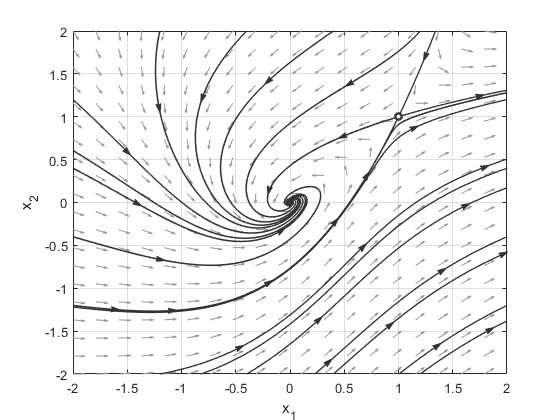
\includegraphics[width=0.7\linewidth]{fig/przyklad_2.png}
            \caption{Portret trajektorii stanu układu (\ref{eq:example_11_sys_transformed}).}
            \label{fig:przyklad_1}
        \end{figure}

        %-------------------------------------------------------
        \subsubsection{Przykład 2}
        Zbadać stabilność punktów równowagi równania:
        \begin{equation}\label{eq:example_12_sys}
            \ddot{x} + \dot{x} + (x+1)x(x-1) = 0.
        \end{equation}
        W celu analizy stabilności przekształcamy równanie do układu równań przez wprowadzenie zmiennych:
        $$
            x_{1} = x, \, x_{2} = \dot{x} = \dot{x}_{1}.
        $$
        Mamy więc:
        \begin{equation}\label{eq:przyklad_2}
            \left\{
            \begin{array}{l}
                \dot{x}_{1} = x_{2}\\
                \dot{x}_{2} = -(x_{1} + 1)x_{1}(x_{1} - 1)- x_{2}
            \end{array}
            \right\}.
        \end{equation}
        Punkty równowagi szukamy przyrównując prawą stronę układu równań (\ref{eq:przyklad_2}) do zera:
        \begin{enumerate}
            \item $x_{e}^{1} = \begin{bmatrix} 0 & 0 \end{bmatrix}^{T}$:
            Przybliżenie liniowe można uzyskać poprzez przybliżenie szeregiem Taylora:
            $$
                \begin{bmatrix} \dot{x}_{1} \\ \dot{x}_{2} \end{bmatrix}
                =
                \frac{\partial f}{\partial x}|_{x_{e}^{1}} + r(x)
                =
                \begin{bmatrix} 0 & 1 \\ 1 & -1 \end{bmatrix}
                \begin{bmatrix} x_{1} \\ x_{2} \end{bmatrix}
                +
                \begin{bmatrix} 0 \\ -x_{1}^{3} \end{bmatrix}
            $$
            gdzie:
            \begin{itemize}
                \item $A = \begin{bmatrix} 0 & 1 \\ 1 & -1 \end{bmatrix}$,
                \item $r(x) = \begin{bmatrix} 0 & x_{1}^{3} \end{bmatrix}^{T}$ i $\lim_{\lVert x \rVert \rightarrow 0}\frac{\lVert r(x) \rVert}{\lVert x \rVert} = \lim_{\lVert x \rVert \rightarrow 0}\frac{|x_{1}^{3}|}{\lVert x \rVert} = 0$.
            \end{itemize}
            Badamy zatem wartości własne macierzy $A$:
            $$
                \begin{vmatrix} \lambda & -1\\ 1 & \lambda + 1 \end{vmatrix} = \lambda^{2} + \lambda - 1 = 0
            $$
            jeden pierwiastek jest dodatni, a drugi ujemny, zatem $x_{e}^{2}$ jest niestabilnym punktem równowagi typu siodło.
            
            \item $x_{e}^{2} = \begin{bmatrix} 1 & 0 \end{bmatrix}^{T}$:
            Aby móc zastosować pośrednią metodę Lapunowa przesuwamy punkt równowagi do początku układu współrzędnych: $z_{1} = x_{1} - 1$, $z_{2} = x_{2}$. Wówczas układ (\ref{eq:example_11_sys_transformed}) przybiera formę:
            $$
                \left\{
                \begin{array}{l}
                     \dot{z}_{1} = z_{2}\\
                     \dot{z}_{2} = -z_{2} - z_{1}^{3} - 3z_{1}^{2} - 2z_{1}
                \end{array}
                \right\}.
            $$
            Więc badany układ można zapisać w postaci (\ref{eq:sys_slabo_niel}) z \textbf{twierdzenia 2}:
            $$
                \begin{bmatrix} \dot{z}_{1} \\ \dot{z}_{2} \end{bmatrix}
                =
                \begin{bmatrix} 0 & 1 \\ -2 & -1 \end{bmatrix}
                \begin{bmatrix} z_{1} \\ z_{2} \end{bmatrix}
                +
                \begin{bmatrix} 0 \\ -3z_{1}^{2} - z_{1}^{3} \end{bmatrix}
            $$
            gdzie:
            \begin{itemize}
                \item $A = \begin{bmatrix} 0 & 1 \\ -2 & -1 \end{bmatrix}$,
                \item $r(z) = \begin{bmatrix} 0 \\ -3z_{1}^{2} - z_{1}^{3} \end{bmatrix}$ i $\lim_{\lVert z \rVert \rightarrow 0}\frac{\lVert r(z) \rVert}{\lVert z \rVert} = 0$.
            \end{itemize}
            Badamy zatem wartości własne macierzy $A$:
            $$
                \begin{vmatrix} \lambda & -1\\ 2 & \lambda + 1 \end{vmatrix} = \lambda^{2} + \lambda + 2 = 0.
            $$
            Pierwiastki równania mają części rzeczywiste ujemne, zatem $x_{e}^{2}$ jest asymptotycznie stabilnym punktem równowagi.
            
            \item $x_{e}^{3} = \begin{bmatrix} -1 & 0 \end{bmatrix}^{T}$:
            Aby móc zastosować pośrednią metodę Lapunowa przesuwamy punkt równowagi do początku układu współrzędnych: $z_{1} = x_{1} + 1$, $z_{2} = x_{2}$. Wówczas układ (\ref{eq:example_11_sys_transformed}) przybiera formę:
            $$
                \left\{
                \begin{array}{l}
                     \dot{z}_{1} = z_{2}\\
                     \dot{z}_{2} = -z_{2} - z_{1}^{3} - 3z_{1}^{2} - 2z_{1}
                \end{array}
                \right\}.
            $$
            Więc badany układ można zapisać w postaci (\ref{eq:sys_slabo_niel}) z \textbf{twierdzenia 2}:
            $$
                \begin{bmatrix} \dot{z}_{1} \\ \dot{z}_{2} \end{bmatrix}
                =
                \begin{bmatrix} 0 & 1 \\ -2 & -1 \end{bmatrix}
                \begin{bmatrix} z_{1} \\ z_{2} \end{bmatrix}
                +
                \begin{bmatrix} 0 \\ -3z_{1}^{2} - z_{1}^{3} \end{bmatrix}
            $$
            gdzie:
            \begin{itemize}
                \item $A = \begin{bmatrix} 0 & 1 \\ -2 & -1 \end{bmatrix}$,
                \item $r(z) = \begin{bmatrix} 0 \\ -3z_{1}^{2} - z_{1}^{3} \end{bmatrix}$ i $\lim_{\lVert z \rVert \rightarrow 0}\frac{\lVert r(z) \rVert}{\lVert z \rVert} = 0$.
            \end{itemize}
            Badamy zatem wartości własne macierzy $A$:
            $$
                \begin{vmatrix} \lambda & -1\\ 2 & \lambda + 1 \end{vmatrix} = \lambda^{2} + \lambda + 2 = 0.
            $$
            Pierwiastki równania mają części rzeczywiste ujemne, zatem $x_{e}^{3}$ jest asymptotycznie stabilnym punktem równowagi.
        \end{enumerate}

        Portret fazowy przedstawiony na rysunku (\ref{fig:przyklad_2}) potwierdza powyższe wnioski.
        \begin{figure}[H]
            \centering
            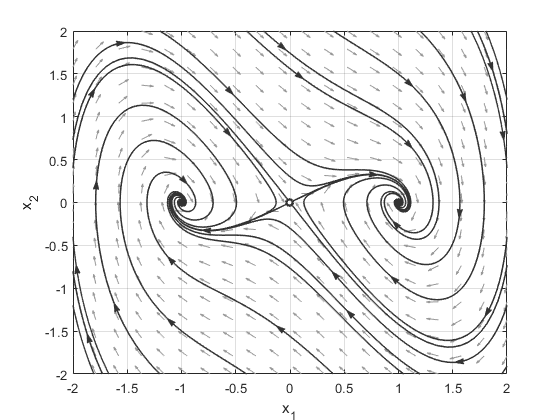
\includegraphics[width=0.7\linewidth]{fig/przyklad_1.png}
            \caption{Portret fazowy układu (\ref{eq:przyklad_2}).}
            \label{fig:przyklad_2}
        \end{figure}

%%%%%%%%%%%%%%%%%%%%%%%%%%%%%%%%%%%%%%%%%%%%%%%%%%%%%%%%%%%% 
\section{Jak to zrobić w MATLABie?}
    %=======================================================
    \subsection{Rozwiązanie macierzowego równania Lapunowa}
    MATLAB dostarcza w toolboxie Control System funkcję rozwiązującą numerycznie macierzowe równanie Lapunowa (\ref{eq:rownanie_lapunowa}).
    Jest to funkcja:
    \begin{lstlisting}[style=Matlab-editor]
        P = lyap(A, Q);
    \end{lstlisting}
    gdzie: \texttt{A} jest macierzą stanu układu liniowego, natomiast natomiast \texttt{Q} jest symetryczną macierzą dodatnio określoną.

    %=======================================================
    \subsection{Symboliczne obliczenia macierzy Jacobiego}
    MATLAB dostarcza poprzez Symbolic Toolbox funkcje do symbolicznego wyznaczania macierzy Jacobiego funkcji nieliniowej:
    \begin{lstlisting}[style=Matlab-editor]
        % Definiowanie zmiennych symbolicznych
        syms x1 x2 x3

        % Dodawanie zalozen o zmiennych symbolicznych
        assume([x1 x2 x3], 'real')   % Zakladamy, ze x1, x2 i x3 przyjmuja tylko wartosci rzeczywiste

        % Definiujemy model nieliniowy
        f = [x2; x3; x1^2 * x3 - x3^3];

        % Wyznaczamy macierz Jacobiego
        A = jacobian(f,[x1, x2, x3]);
    \end{lstlisting}


    %=======================================================
    \subsection{Wyznaczanie trajektorii bez Simulinka}
    MATLAB dostarcza kilku funkcji służących do numerycznego rozwiązywania równań różniczkowych.
    Jedną z nich jest \texttt{ode45}, rozwiązująca równanie metodą Rungego-Kutty 4. rzędu.
    \begin{lstlisting}[style=Matlab-editor]
        model_dynamiki = @(t,y)[x(2); -x(1) + x(2)x(1)^3];
        tspan = 0 : 0.01 : 10;
        y0 = [1; 1];
        
        [y, t] = ode45(model_dynamiki, tspan, y0);
    \end{lstlisting}
    Innymi funkcjami, rozwiązującymi równania różniczkowe, są np.: \texttt{ode23}, \texttt{ode113}.

%%%%%%%%%%%%%%%%%%%%%%%%%%%%%%%%%%%%%%%%%%%%%%%%%%%%%%%%%%%%
\newpage
\begin{thebibliography}{9}

\bibitem{Mitkowski2007}
  Mitkowski W., Baranowski J., Hajduk K., Korytowski A., Tutaj A.,
  \emph{Teoria Sterowania: Materiały Pomocnicze do Ćwiczeń Laboratoryjnych},
  AGH Uczelniane wydawnictwo Naukowo-Dydaktyczne,
  2007.

\bibitem{Mitkowski2019}
    Mitkowski W.,
    \emph{Zarys Teorii Sterowania},
    Wydawnictwa AGH,
    2019.

\bibitem{Amborski1978}
  Amborski K., Marusak A.,
  \emph{Teoria Sterowania w Ćwiczeniach},
  Państwowe Wydawnictwo Naukowe,
  1978.

\bibitem{Gessing1981}
  Gessing R., Latarnik M., Skrzywan-Kossek A.,
  \emph{Zbiór Zadań z Teorii Nieliniowych Układów Regulacji i Sterowania},
  Wydawnictwo Naukowo-Techniczne,
  1981.

\bibitem{Gibson1968}
  Gibson J. E.,
  \emph{Nieliniowe Układy Sterowania Automatycznego},
  Wydawnictwo Naukowo-Techniczne,
  1968.

\bibitem{Kabzinski2018}
  Kabziński J., Mosiołek P.,
  \emph{Projektowanie Nieliniowych Układów Sterowania},
  Wydawnictwo Naukowo PWN,
  2018.

\bibitem{LaSalle1966}
  La Salle J., Lefschetz S.,
  \emph{Zarys Teorii Stabilności Lapunowa i Jego Metody Bezpośredniej},
  PWN,
  1966.

\bibitem{Shinners1992}
  Shinners S. M.,
  \emph{Modern Control System Theory and Design},
  Wiley \& Sons,
  1992.

\bibitem{Kaczorek2005}
  Kaczorek T.,
  \emph{Podstawy Teorii Sterowania},
  Wydawnictwo Naukowo-Techniczne,
  2005.

\bibitem{Chang2019}
  Chang Y-C., Roohi N., Gao S., 
  \emph{Neural Lyapunov Control},
  33rd Conference on Neural Information Processing Systems, Vancouver, Canada.,
  2019.

\bibitem{Dai2021}
  Dai H., Landry B., Yang L., Pavone M. i Tedrake R.,
  \emph{Lyapunov-stable neural-network control},
  Robotics: Science and Systems ,
  2021.

\end{thebibliography}

\end{document}
